\documentclass[a4paper,10pt]{article}
\usepackage[a4paper,bindingoffset=0.2in,%
            left=1in,right=1in,top=1in,bottom=1in,%
            footskip=.25in]{geometry}
\usepackage[english]{babel}
\usepackage{helvet}
\usepackage{cmbright}
\usepackage{authblk}
\usepackage{graphicx}
\usepackage{amssymb}
\usepackage{url}
\usepackage{bm}
\providecommand{\keywords}[1]{\textbf{\textit{Keywords ---}} #1}
 
\title{Introduction to the methods for classification}

\begin{document}
\sffamily
\maketitle

In many fields, research teams aim to model data for purposes going from better understanding of our world to prediction of the future.
Although, historically, these problems were only tackled through statistical modeling, in the last decade, machine learning gained popularity. Indeed, machine learning is the branch of computer science that uses past experiences to take future decisions without a complete knowledge of all influencing elements \cite{bonaccorso2017machine}. Machine learning techniques can be divided in three main categories: supervised learning, unsupervised learning and reinforcement learning. In supervised approaches, such as classification or regression, the relationships between data and a targeted output are taught beforehand whereas for unsupervised techniques (e.g., clustering) relations and hidden patterns in data are independently found. Afterwards, both approaches can be included in reinforcement learning where the model will continue to learn from environment feedback.

The world of machine learning is wide and is still in expansion. It would be difficult to go through all underlying concepts of artificial intelligence, and thus, this article mainly focuses on one aspect of machine learning: supervised learning for classification.

%Indeed, we saw in Sections \ref{Motioncharacterization} and \ref{AudioClassif} of Chapter 2, that classification is a valuable tool to clinically characterize newborn conditions either to recognize motion patterns or to classify cries. 
%During this thesis, methods for classification were applied in order to tackle three problems: sleep stages classification, motion segmentation and cry extraction.

\section{Problem formulation}
\label{Formulation}
The term "classification" covers all techniques that classify data into a given number of classes. Being part of the supervised branch of machine learning, classification requires a learning phase on labeled data to identify in which class a new data sample belongs to \cite{joshi2017artificial}. Therefore, for classification problems, data has to be formed by the pair $(\bm{X},Y)$\footnote{Matrices are noted in bold capital letters and vectors with capital letters} with the data description matrix $\bm{X}$ of size $N$ x $p$ and the set of labels $Y$ $\in$ $\left\{c_1, \ldots, c_k\right\}$, where $k$ is the number of targeted classes, $N$ is the number of labeled samples and $p$ is the number of features which characterize each sample. More precisely, each sample $i$ of the data is described through the feature set $X_i = [x_{i1}, x_{i2}\ldots, x_{ip}]$.
This is depicted and illustrated by an example in Figure~\ref{dataForm}.

\begin{figure}[htbp]
\centerline{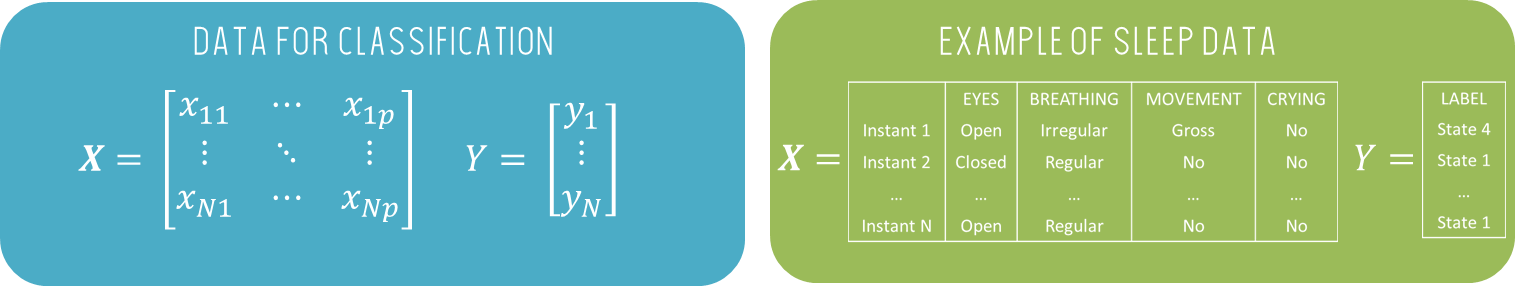
\includegraphics[width=\linewidth]{./figures/data.png}}
\caption{Data for classification summary (left), supplemented by a sleep state dataset example (right).}
\label{dataForm}
\end{figure}

Visually, each line of $\bm{X}$ contains the feature set of dimension $p$ that describe a sample. A sample is associated with an output class which is reported in $Y$ at the corresponding line. Hence, in the example, sleep data is formed by the pair $(\bm{X},Y)$, where $\bm{X}$ is composed by $N$ instants. Four qualitative features are used to describe each instant ($=$ sample): Eyes, Breathing, Movement and Crying ($p=4$). Associated sleep states are contained in $Y$. Sleep states are labeled from 1 to 5 ($k=5$), as defined in Chapter~1.
In the sleep dataset example, only qualitative features (i.e, descriptive) are presented although quantitative features (i.e., numeric) can also be integrated into $\bm{X}$.

To construct an accurate classification model, the process, depicted by Figure \ref{processML} and described below, is generally followed \cite{dangeti2017statistics}. It implies five steps: collection of the data, feature engineering, learning, testing and deployment.

\begin{figure}[htbp]
\centerline{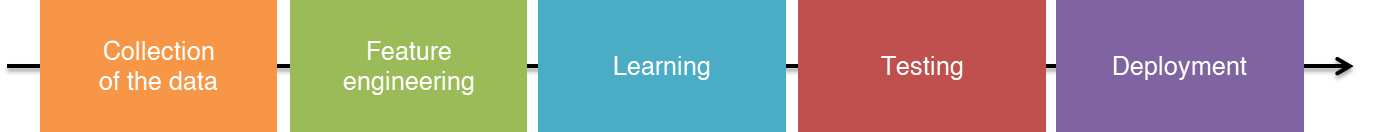
\includegraphics[width=\linewidth]{./figures/process.png}}
\caption{Overview of the classification process from data collection to deployment.}
\label{processML}
\end{figure}

In fact, it is necessary to keep in mind these steps to avoid two major problems of machine learning: underfitting and overfitting.
Underfitting characterizes a model which fails to generalize the data, usually, due to a lack of training samples. Reversely, overfitting occurs when a classifier corresponds too closely or exactly to a particular set of data and fails to fit future data.

\paragraph{Collection of data} 
The data collection is an important step to construct an accurate classification model. The more various are the training samples, the better will be the classification when deploying the model. It is important to notice that data used to train are the only knowledge of the model and thus, if a given event is too much represented in the data, the model may overfit.

\paragraph{Feature engineering}
One of the main challenges of classification is to provide an informative set of features regarding the targeted outputs of the model. In some cases, data may have to be processed first to extract describing features. One can think that the more features are extracted the better will be the model. However, a large big set of features can also lead to overfitting. This effect is known as the curse of dimensionality \cite{tang2014feature}. To overcome this issue, it is sometimes necessary to reduce the feature set dimension $p$. To do so, several techniques exist and are presented in Section~\ref{dimension}.

\paragraph{Learning phase}
Once data have been prepared, the learning phase can be initiated. Most of the machine learning techniques depend on parameters and/or hyper-parameters\footnote{To avoid confusion, the use of "parameter" and "hyper-parameter" has been dedicated to mention the setting of methods whereas the term "feature" is exclusively associated with data either when it is question of raw features or after computation.} that need to be tuned to better fit the data (see  Section \ref{MLtech}). During the learning phase two datasets are usually used: the training and the validation dataset. We will see in Section \ref{Evaluation} that several approaches exist to divide the data to obtain both sets. In machine learning, parameters are tuned by covering a large scale of possible values and integrating them into the learning phase. Then, trained model is applied on the validation set and the set of parameters that will be retained is the one giving the best performances regarding the objective of classification. As the way of looking performances can change regarding the application, further details on this question are provided in Section \ref{metrics}.

\paragraph{Testing the algorithm on unseen data}
In order to ensure the quality of the model predictions, it is common in machine learning to apply the model on an additional test set of unseen (but labeled) data. This way, if high performances are observed at the learning phase but a poor generalization is observed on the test set, it is a direct indicator of overfitting.

\paragraph{Deployment of the algorithm}
The last step of the process is to deploy the algorithm in order to make predictions on unlabeled real data. Normally, if the model has been correctly evaluated on a test set independently of the training phase, future classifications would be accurate. However, it can happen that the performances may be altered. Indeed, the annotated data, inherently to conditions of collection, can be unreliable to infer the whole population. Although it is a tough question to ensure a totally random and independent collection of data, it is important to keep in mind this limitation \cite{mitData}.
\\
\\
In the following sections, further details are provided about dimensionality reduction methods, machine learning algorithms and evaluation techniques used for classification. An overview of the methods mentioned hereafter is proposed by Figure \ref{mindmapML}.

\section{Dimensionality reduction}
\label{dimension} 

Dimensionality reduction is the process of reducing the size of the feature set. Although this step is not mandatory, when the data are described by many features, performing dimensionality reduction is a good trick for, among others, the following reasons \cite{coelho2015building}:
\begin{itemize}
\item Reduce the risk of overfitting;
\item Speed up the learning phase;
\item Lower the model computational complexity;
\item Visualize data using a limited number of dimensions.
\end{itemize}

\begin{figure*}[htbp]
\vspace{3cm}
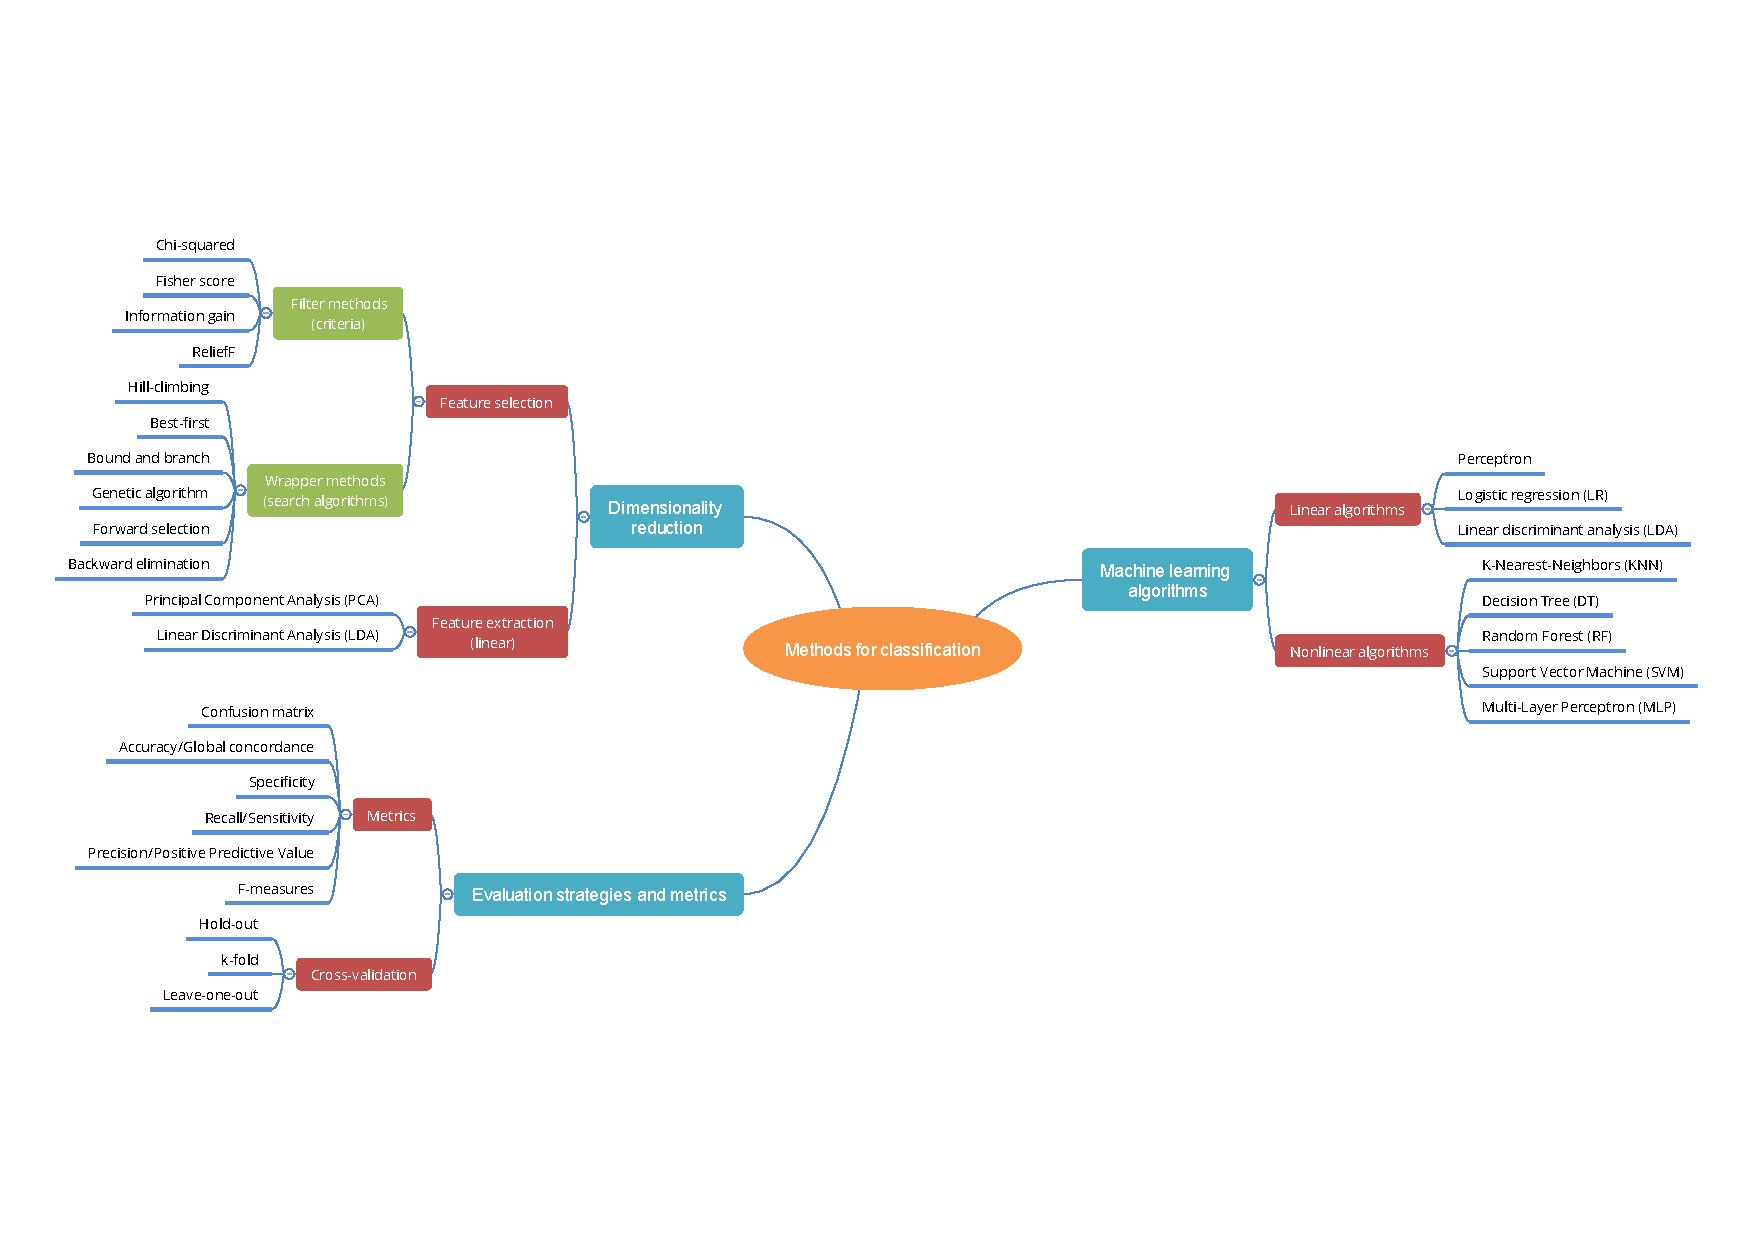
\includegraphics[width=\linewidth]{./figures/mindmapML.pdf}
\vspace{1cm}
\caption{Overview of methods for classification.}
\label{mindmapML}
\end{figure*}

In practice, two main groups of dimensionality reduction methods are used: feature selection and feature extraction, sometimes also called feature projection. The main difference between these approaches is that feature extraction maps the original feature space into a lower-dimensional space while, in feature selection, a subset of the original feature set is selected. The choice to use either selection or extraction methods can depend on the objective of the model. If the objective is to better understand the influence of features on classes, feature selection is more suited. Indeed, in feature extraction, the new feature set obtained by projection is generally difficult to link with physical meaning \cite{tang2014feature}.

\subsection{Feature selection}

Feature selection methods are used to select features that are the most suitable to discriminate samples that belong to different classes. Hence, the goal is to find the best subset of features among the $2^p$ candidate subsets \cite{dash1997feature}.

Generally, the selection approach, depicted by Figure \ref{processFeatureSelection}, combines feature subset evaluation and search algorithm. Several iterations are performed to search the best subset. For each iteration, a subset is evaluated and its "goodness" is returned. 

\begin{figure}[htbp]
\centerline{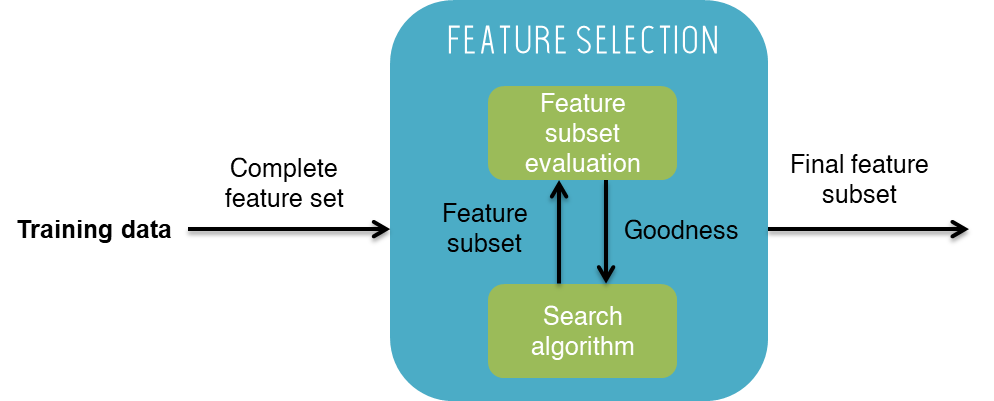
\includegraphics[width=0.6\linewidth]{./figures/featureselection.png}}
\caption{Framework of feature selection methods.}
\label{processFeatureSelection}
\end{figure}

When the original feature set is large, looking for all possibilities is greedy. Hence, computational complexity of the search can be reduced by heuristic or randomized methods to prevent an exhaustive search. These methods are associated with a stopping criterion on the "goodness".

The "goodness" criterion depends on the applied method and objectives. Two main categories of methods stand out: filter models or wrapper models. In the filter approach, the "goodness" is related to information content of the subset while, in wrapper, it is the predictive performances, obtained on the validation set with the subset of features that is evaluated.

\subsubsection{Filter methods}

Filter models rely on the characteristics of the data without using any classification method \cite{liu2007computational}. Typically, features are ranked and the highest ranked ones are selected. This can be done in two ways: univariate or multivariate. In the univariate scheme, each feature is ranked independently from others whereas all features are considered simultaneously in the multivariate approach. Several criteria have been applied to rank data. Among them, we can cite: quality (Fisher score \cite{duda2012pattern,gu2012generalized}), independency (Chi-squared \cite{bonaccorso2017machine}), redundancy (information gain \cite{roobaert2006information}) or separation of class instances (ReliefF \cite{kira1992feature}).

Since filter models are easy to understand and implement, it is a popular technique. However, features are selected independently from classification and thus, filter models totally ignore the effects of the selected subset on the performance of the classification algorithm \cite{hall1999feature}.

\subsubsection{Wrapper methods}

Wrapper models were developed to overcome the limitation of filter models. The subset evaluation is performed by integrating the classifier. Hence, the subset is adapted to the inherent particularities and bias of a predefined classifier \cite{tang2014feature}.
To find the best subset, a wide range of search strategies exists including hill-climbing, best-first, branch-and-bound, and genetic algorithms \cite{guyon2003introduction}. Two other popular methods are forward selection and backward elimination where features are respectively added or removed one by one.

Wrapper models provide better predictive performances than filter models \cite{kohavi1997wrappers}. Nevertheless, they are more computationally expensive than filter models.

\subsection{Feature extraction}
The concept under feature extraction is to project the original feature set of dimension $p$ into a lower-dimensional space of dimension $m$.

Two types of feature extraction methods can be distinguished depending on the way to combine the features: linear and non-linear. In linear feature extraction methods, new features in the lower dimensional space are given by a linear combination of the original feature set. Reversely, non-linear combinations are sought with non-linear approaches. 
Linear techniques being principally used, this section mainly focuses on this approach.
The main challenge of linear feature extraction methods is to find a transformation $\bm{W}$, such as:
\begin{equation}
\bm{Z} =  \bm{W}^T \bm{X}
\end{equation}
where $\bm{Z}$ is the projected data set of size $m * N$, with $m < p$ and $N$ is the number of samples.
Dimensionality reduction by the mean of linear feature extraction is depicted by Figure \ref{FeatureExtraction} with an example of projection from a space of dimensions $p = 2$ to a space of dimension $m=1$. This example shows that an infinite number of solutions exists to find a new axis to project data points. However, in the literature, two methods stand out: Principal Component Analysis (PCA) and Linear Discriminant Analysis (LDA) \cite{tang2014feature}, described below. 
%The main difference between the two methods is that PCA is an unsupervised approach while LDA is a supervised method, where labeled data are mandatory. 

\begin{figure}[htbp]
\centerline{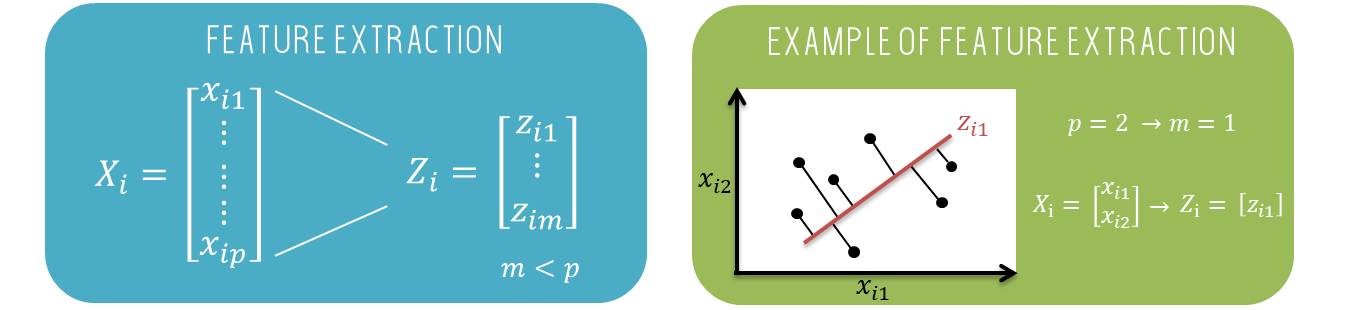
\includegraphics[width=\linewidth]{./figures/featureExtraction.png}}
\caption{Feature extraction concept (left) and associated example (right). $X_i$ is the original feature set describing the sample $i$ and $Z_i$ is the extracted feature set. In the example, black dots represent data in a two-dimensional space and the red line represents an example of axis for projection in a one-dimensional space.}
\label{FeatureExtraction}
\end{figure}

\subsubsection{Principal Component Analysis}

Principal Component Analysis is a well-known technique of data transformation \cite{jolliffe2011principal}. In its standard formulation, it finds the most discriminant projection of the original feature set by maximizing the variance between data points. 
In practice, the eigenvectors of the covariance matrix, calculated from the original feature set, are computed. Then, the ones with the largest eigenvalues (principal components) are used to reconstruct a part of the variance of the original dataset.

After that, there are two ways of using principal components regarding the objective of the analysis. The first one is data visualization. In that case, only two or three principal components, carying most of the variance, will be retrieved in order to plot the data in a two to three dimensional graph. This way, further analyses can be conducted regarding the distribution of data within the objective of class separation. Another purpose of PCA is to feed machine learning algorithms for classification purpose. With PCA, the reduction of dimension can be regulated by the total variance wanted for the feature subset. In other words, the number of principal components that are kept depends on the percent of variance information wanted by the user. 

The main limitation of PCA is that there is no guarantee that a small number of principal components with the highest variance will contain the information needed for the classification \cite{neal2006high}. Hence, relevant information can be lost and the resulting projected features $\bm{Z}$ can lead to weak classification performances.
Additionally, PCA is only suited for quantitative set of feature. Other factor methods exists. Among them we can cite Multiple correspondence analysis \cite{le2010multiple} for qualitative feature set and factor analysis of mixed data for mixed feature set \cite{escofier2008analyses}. Moreover, a version of PCA, called kernel PCA, has been proposed to make non-linear projections \cite{scholkopf1997kernel}. Briefly, an initial step is first performed to find a particular space where the dataset becomes linearly separable \cite{bonaccorso2017machine}.

\subsubsection{Linear Discriminant Analysis}
\label{LDAExtr}
Contrary to PCA, in Linear Discriminant Analysis, labels are integrated in the process of dimension reduction. LDA finds the most discriminant projection by maximizing between-class distance and minimizing the within-class distance \cite{balakrishnama1998linear}.

In practice, the eigenvectors of the between-class and within-class covariance matrices are computed and the best projection is found using Fisher's criterion.
\begin{figure}[htbp]
\centerline{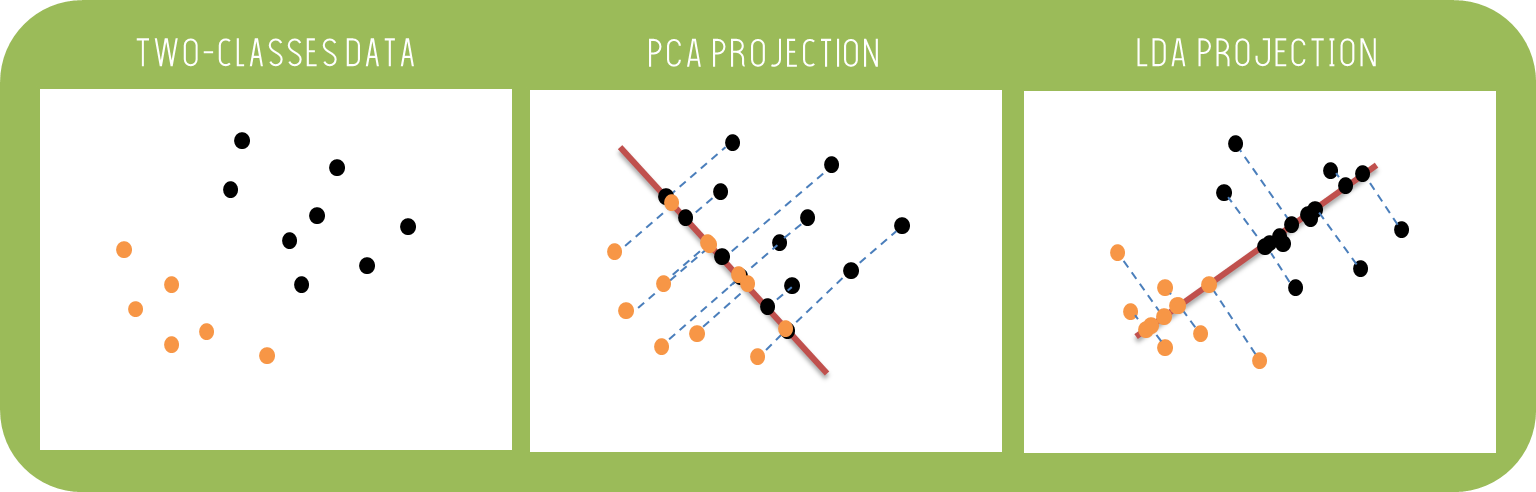
\includegraphics[width=\linewidth]{./figures/comparaisonLDAPCA2.png}}
\caption{Comparison of data projection between Principal Components Analysis and Linear Discriminant Analysis for a two-classes problem. Orange dots represent data of the first class and data belonging to the second class are reported in black. The red line represents the resulting axis for projection obtained for each method.}
\label{CompLDAPCA}
\end{figure}

A comparative example between PCA and LDA is given by Figure \ref{CompLDAPCA}. For a two-class data example, the resulting axis that preserves the variance on the whole data set (PCA) and the one that preserves the distance between both classes (LDA) are drawn. We can see, on each axis, the resulting data projection. LDA offers, in that case, a better projection for discriminating purpose. In fact, besides dimensionality reduction, LDA can also be used for classification (see Section \ref{LDAML}).

\section{Machine learning algorithms}
\label{MLtech}
As mentioned in Section \ref{Formulation}, a supervised machine learning technique is an algorithm that learns from past experiences (training set) a model to make future predictions.

Classifiers\footnote{In classification, machine learning algorithms are also called classifiers.} aim to find the best decision boundaries to discriminate between classes. As illustrated by Figure \ref{LinearVsNonLinear}, there are two types of classification cases: the ones where classes can be separated with linear boundaries and the ones where classes are not linearly separable.

\begin{figure}[htbp]
\centerline{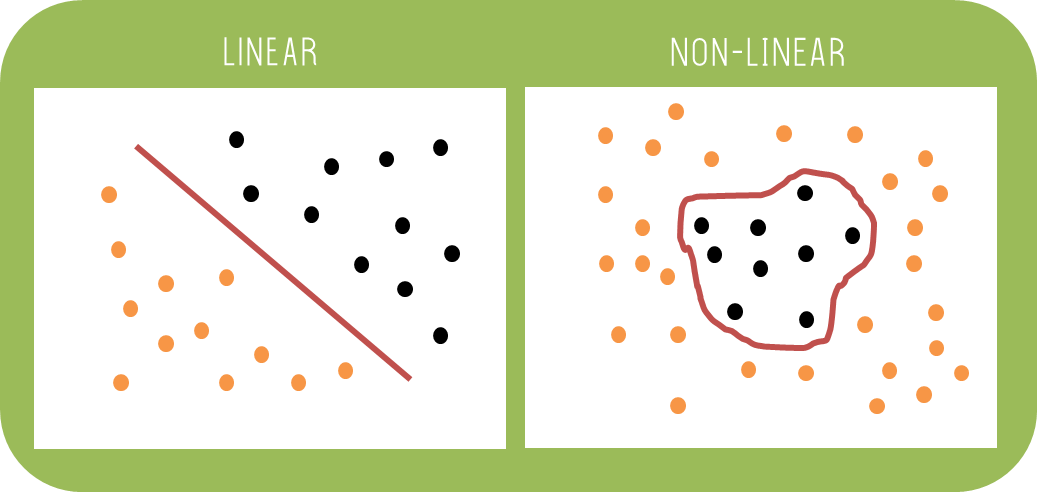
\includegraphics[width=0.65\linewidth]{./figures/LinearNonLinear.png}}
\caption{Illustration of a linearly separable case (left) and a non-linearly separable case (right). Red lines represent examples of boundary decisions.}
\label{LinearVsNonLinear}
\end{figure}

Hence, classifiers can be divided in two groups: linear algorithm and non-linear algorithms. To illustrate the different approaches used to solve classification problems, in this section, we will go through eight commonly used classifiers.

\subsection{Linear algorithms}

Linear classifiers aim to find a linear decision boundary between classes. It can either be a line, a plane or a hyperplane, depending on the dimension of the problem.

\subsubsection{Perceptron}
The most basic linear model is the perceptron \cite{rosenblatt1958perceptron}, depicted in Figure~\ref{Perceptron}.
\begin{figure}[htbp]
\centerline{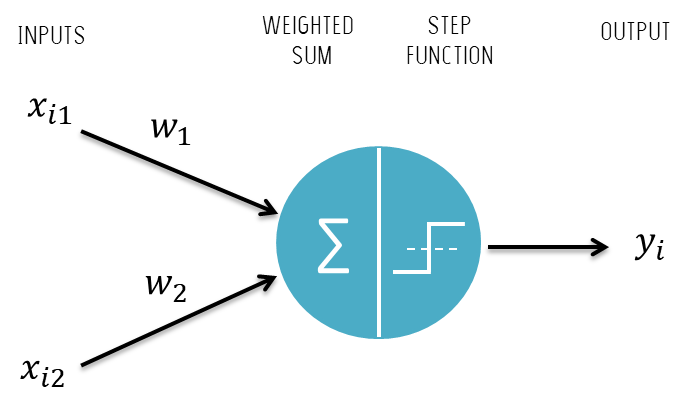
\includegraphics[width=0.4\linewidth]{./figures/perceptron.png}}
\caption{Illustration of a perceptron with two inputs.}
\label{Perceptron}
\end{figure}

In this example, the perceptron output decision $y_i$, which can either be $-1$ or $+1$, is computed for each sample $i$ as:
\begin{equation}
y_i = f(w_1x_{i1} + w_2x_{i2})
\end{equation}
where $f$ is a step function, also called threshold or activation function. This can be generalized for a larger dimension $p$ by:
\begin{equation}\label{linearEquation}
Y = f(W^T\bm{X}+b)
\end{equation}
where $W$ is the weight vector defined as $W = \left\{ w_1, w_2, \ldots, w_p \right\}$ and $b$ is the bias.

To summarize, to make a prediction, the perceptron computes two quantities. First, the weighted sum of the input features is calculated. Then, this sum is thresholded by the function $f$ in order to retrieve a prediction equal to $-1$ or $+1$.

During the training phase, $W$ is firstly randomly initialized. Then, weights are settled by considering all the samples of the training set and looking at the output decision \cite{shiffman2012nature}. It is performed in three steps which are repeated until all training samples are correctly classified:
\begin{enumerate}
\item Make a prediction for an input sample;
\item Compute the error $\epsilon$ between the prediction and real label;
\item Adjust the new vector of weights $W'$ accordingly to the error, such as:
\begin{equation}
W' = W + \Delta W
\end{equation}
\end{enumerate}
where $\Delta W =$ $\epsilon$ x $\eta$ x $X_i$, with $\eta$, called the learning rate\footnote{It is used to regulate the scale of the weight modifications.} and $X_i$, the input features of the sample.

So far, we presented a two-class classification approach. In case of multiclass problems, several perceptrons can be trained in order to predict each class versus all others (one-versus-the-rest).

The power of perceptron classifiers resides in the fact that if a linear boundary exists to discriminate classes, the model will converge perfectly. However, in most classification problems, an overlap exists between classes and perceptron models will necessary present misclassification. 

\subsubsection{Logistic Regression}

Logistic Regression (LR) is quite similar to perceptron except that instead of a class prediction, it returns a probability of belonging to the positive class. Hence, in some cases, it may be more robust to class overlap. 
To compare between perceptron and logistic regression lets restart from Equation (\ref{linearEquation}). In logistic regression, $b$ is commonly renamed $w_0$, the model intercept. Then, for each sample, a score $S(X_i)$ is computed as:
\begin{equation}
S(X_i) = f(W^TX_i+w_0)
\end{equation}

In logistic regression, $f$ is fixed and is called the logistic (or sigmoid) function. The sigmoid function, depicted by Figure~\ref{sigmoid}, is used to associate each score to a probability bounded between $0$ and $1$, such as:
\begin{equation}
P(Y_i) = f(S(X_i))
\end{equation}

\begin{figure}[htbp]
\centerline{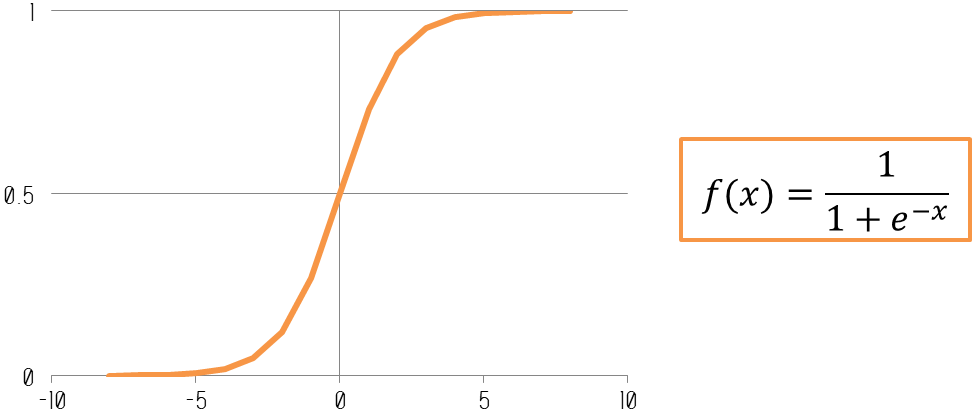
\includegraphics[width=0.6\linewidth]{./figures/sigmoid.png}}
\caption{Sigmoid function.}
\label{sigmoid}
\end{figure}

After that, a cut-off value is usually applied on the probability to obtain the class output.

In the learning phase, the vector of weights $W$ has to be estimated. Here, the best $W$ is the one that maximizes the conditional probabilities $P(Y|\bm{X}, W)$ on the training set. This is commonly done by Maximum Likelihood Estimation (MLE), based on the assumption that weights are normally distributed \cite{czepiel2002maximum}.

Logistic regression is usually applied for binary classification. However, as well as perceptron, it is possible to extend it to multiclass problems by training several one-versus-the-rest LR classifiers.

\subsubsection{Linear Discriminant Analysis}
\label{LDAML}

As mentioned in Section \ref{LDAExtr}, Linear Discriminant Analysis can be used for feature extraction. It can also be applied for classification purpose. Contrary to previous linear methods, LDA is more suited for multiclass analysis \cite{rao1948tests}. We saw that LDA aims to find the best projection by maximizing the mean between-class distances while minimizing the within-class variance. For multiclass problems, a initial step is added to compute the overall mean (= center) of the data. Then, it is the distance between each class and this center that is maximized while minimizing the within-class variance. 

In this way, distributions (means and variance) of each class are estimated. Thus, by the use of Bayes' theorem, the probability of a sample to belong to each class can be estimated. For future predictions, the class associated with the higher probability will be returned.

Nevertheless, LDA presents two main limitations. The first one is due to the number of samples for each class in the training set. If a class is under-represented, the estimated distribution for this class will be corrupted. Secondly, as previous methods, LDA is more suitable on linearly separable multiclass problems.

\subsection{Non-linear algorithms}

In case of non-linear problems, where class boundaries cannot be approximated by hyperplanes, non-linear algorithms may be more reliable than linear classifiers. 

\subsubsection{K-Nearest Neighbors}

K-Nearest Neighbors is a basic method used for classification. Basically, it computes all the distances between a new sample and the ones of the training set. Then, the majority class of its neighbors is assigned to it. The number of neighbors that contributes to the vote is determined by $k$.

\begin{figure}[htbp]
\centerline{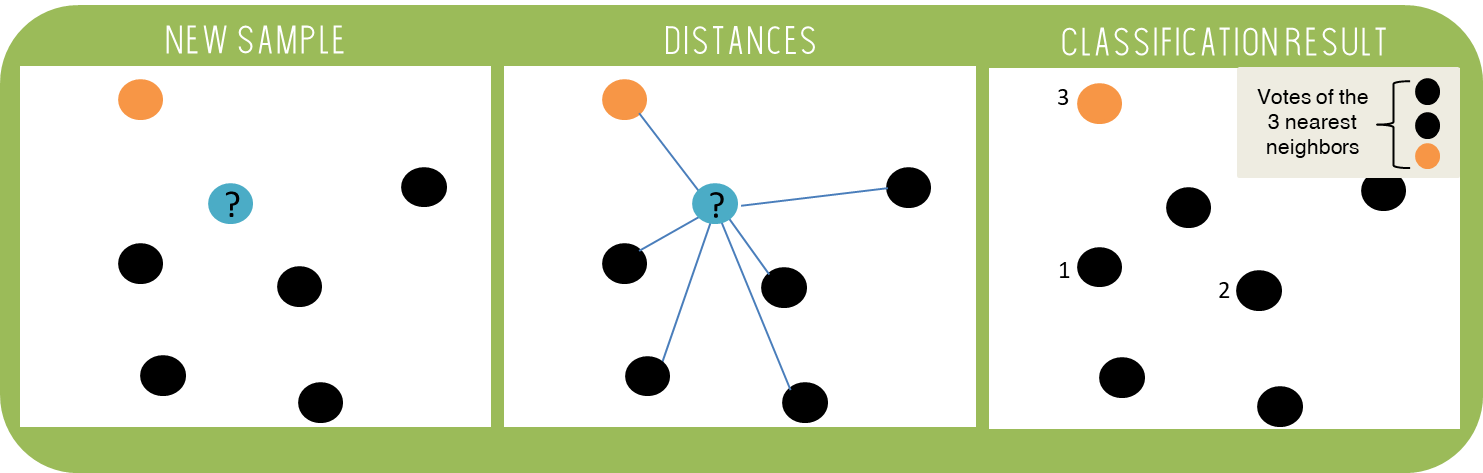
\includegraphics[width=\linewidth]{./figures/KNNIlustration.png}}
\caption{Example of K-nearest neighbors classification with $k=3$.}
\label{KNNEx}
\end{figure}

An example of KNN classification, with $k=3$, is given by Figure \ref{KNNEx}. In this example, the class of a new sample (in blue) is sought. The distance with all others points of the learning set is computed. Labels of the 3 nearest neigbours are checked. With two neighbors belonging to class "Black" and one to class "Orange", the new sample is classified as a "Black" sample.

Although Hamming, Manhattan or Minkowski distances can be used, KNN classifier is commonly based on the Euclidean distance.
The Euclidean distance between a sample of the training set $X_{i}$ and a new sample $X_{n}$, is computed as:
\begin{equation}
d(X_{i},X_{n}) = \sqrt{(x_{i1}-x_{n1})^2+(x_{i2}-x_{n2})^2+\ldots+(x_{ip}-x_{np})^2}
\end{equation}
To compute an accurate distance, it is necessary to work on homogeneous features (i.e., with the same scale). Indeed, absolute differences in features must weight the same to avoid the computation of a meaningless distance.

KNN is a popular algorithm in classification due to its simplicity. In fact, the algorithm is intuitive and easy to implement. Additionally, it can perform well for both linear and non-linear cases. 

However, KNN has some drawbacks. It is easily subject to overfitting, especially when working with an imbalanced training dataset \footnote{when the proportion of samples for a class is high or low in comparison with others}. In addition, it can require a lot of memory for future predictions since it needs the training data samples to compute distances.

\subsubsection{Decision tree}
\label{DT}
Decision tree is a predictive model approach which is constructed as a tree-shaped diagram, composed by nodes, branches and leaves. It provides the statistical probability of a class to occur. An example of tree architecture, for a four classes problem and a feature set of three components, is provided in Figure~\ref{TreeEx}.

\begin{figure}[htbp]
\centerline{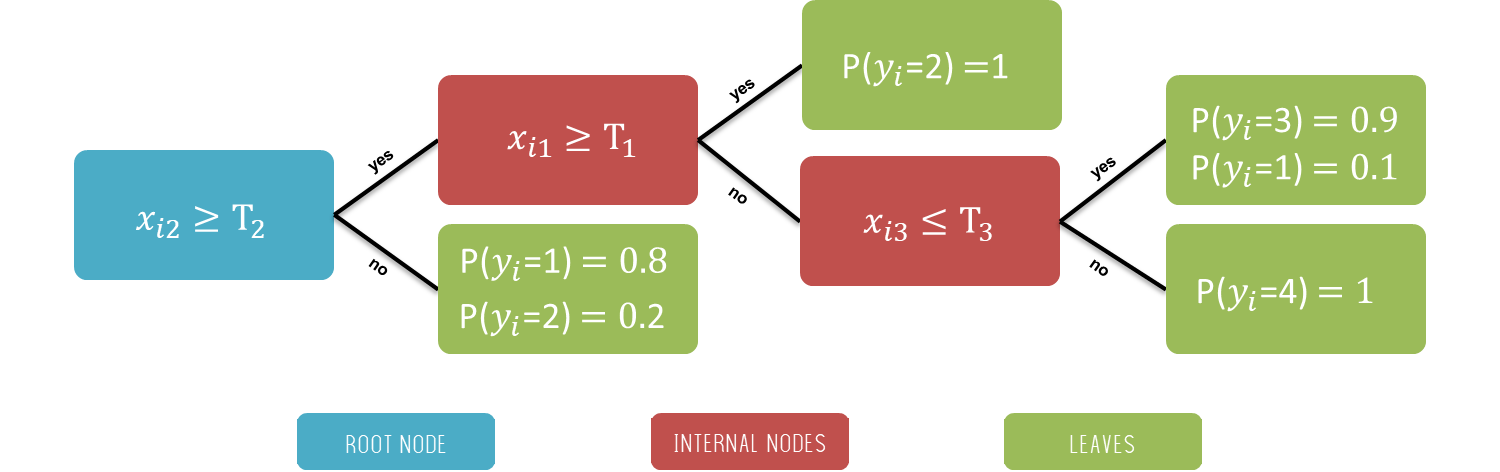
\includegraphics[width=0.8\linewidth]{./figures/DT.png}}
\caption{Tree architecture for a four classes examples, where $x_{i1}$, $x_{i3}$ and $x_{i3}$ are the feature set of a sample $i$ and $y_i$ is the predicted class. $T_1$, $T_2$, $T_3$ are three thresholds.}
\label{TreeEx}
\end{figure}

The prediction for a new sample is given using a succession of small tests. Each node corresponds to a test until a leaf, giving the overall output decision, is reached. Hence, in the tree example, if a new data sample $n$ has:
\begin{itemize}
\item its feature $x_{n2}$ is superior to $T_2$;
\item its feature $x_{n1}$ is inferior to $T_1$; 
\item its feature $x_{n3}$ is inferior to $T_3$.
\end{itemize}
Then, there is a probability of 0.9 that it belongs to class 3 and a probability of 0.1 to belong to class 1. Generally, the highest probability is retained, making "class 3" the final decision for this sample.

In the training phase, two elements are determined: the architecture (e.g., the order of the considered features, the number of nodes and leaves) and threshold for each feature.
A decision tree is constructed following these steps:
\begin{enumerate}
\item Split the training set by thresholding a feature;
\item Compute a measure of the quality of the split;
\item Repeat Step 1 and Step 2 until all the splitting possibilities (all thresholds for all features that wasn't used in previous nodes) are associated with a quality measurement;
\item If the split with the best quality measurement improves the classification of the previous node, it is a new node. Otherwise, the previous node was better and is turned into a leaf.
\item Repeat all the previous steps until only leaves can be reached.
\end{enumerate}

To measure the quality of a split, a criterion based on impurity (e.g., Gini's) or information gain (e.g., entropy) can be used \cite{dangeti2017statistics}. In practice, it is often the Gini's impurity that is applied:
\begin{equation}
Gini = 1 - \sum_{c=1}^C P(c)^2
\end{equation}
where $C$ is the number of classes and $P(c)$ is the fraction of samples of class $c$ observed after the split. The lower is the Gini's criterion, the better is the split.

Decision trees are easy to understand and interpret. Additionally, they require very few data preparation (such as scaling in KNN) since splits are independently made for each feature. However, they can easily lead to overfitting if the set of features is too wide. As KNN, they are also sensitive to imbalanced dataset since the number of samples in each class impacts the quality criterion.

\subsubsection{Random Forests}

Random Forest is a part of "ensemble methods" of machine learning. Ensemble methods are based on the assumption that diversified and independent models tend to give better classification results. Therefore, Random Forest is a combination of tree predictors \cite{breiman2001random}. The classification result comes from the majority vote of a collection of decision trees (also called bagging). In fact, it aims to enhance the generalization by averaging multiple decision trees trained on different parts of the same training set. Figure~\ref{RFEx} shows the workflow for a new prediction with a RF model of $E$ trees.

\begin{figure}[htbp]
\centerline{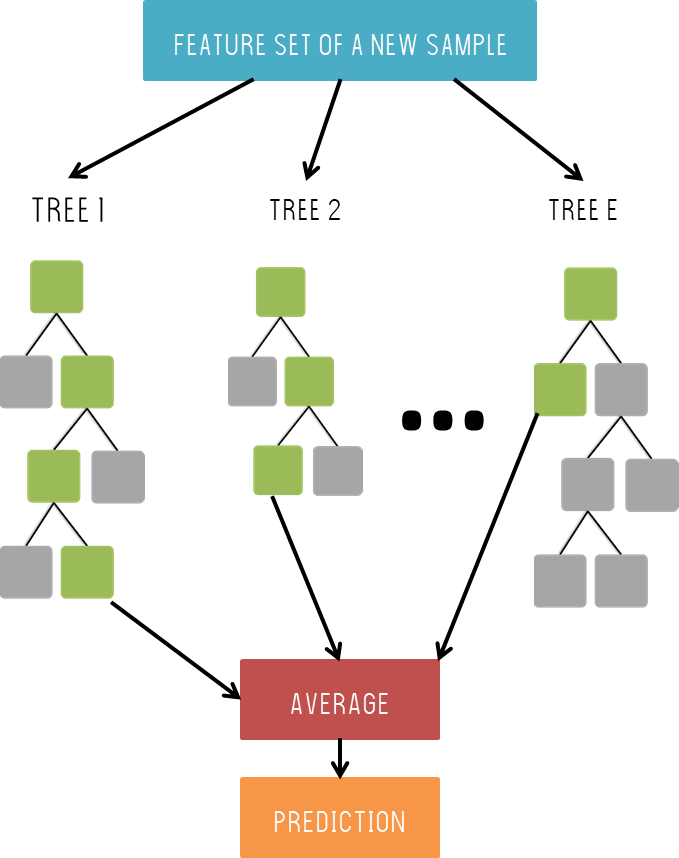
\includegraphics[width=0.4\linewidth]{./figures/RF.png}}
\caption{Prediction workflow with a Random Forest model composed by $E$ trees. Successive test results for each tree are reported in green.}
\label{RFEx}
\end{figure}
 
In the learning phase, each tree is growing, as described in Section \ref{DT}, from a randomly selected subset of the feature set. In this way, each tree is growing with different features. Indeed, if the whole feature set was used, significant features would always come first in the top nodes of splitting which would make all trees be more or less similar.

Random forest is a very popular learning method that can reach really high performances. Contrary to previous methods, it can be robust to imbalanced dataset since a prior knowledge of class occurrences can be integrated in the algorithm. However, results are difficult to interpret since it can be constructed with hundreds of trees. Additionally, sometimes, RF can overfit due to a too noisy dataset (i.e., with a lot of outliers/extreme cases).

\subsubsection{Support Vector Machines}

Support Vector Machines are suited for both linear and non-linear problems \cite{cortes1995support}. The aim of SVM is to find the hyperplane boundary that leaves the maximum margin between two classes. Figure~\ref{SVMEx} illustrates the SVM terminology on a linear example.

\begin{figure}[htbp]
\centerline{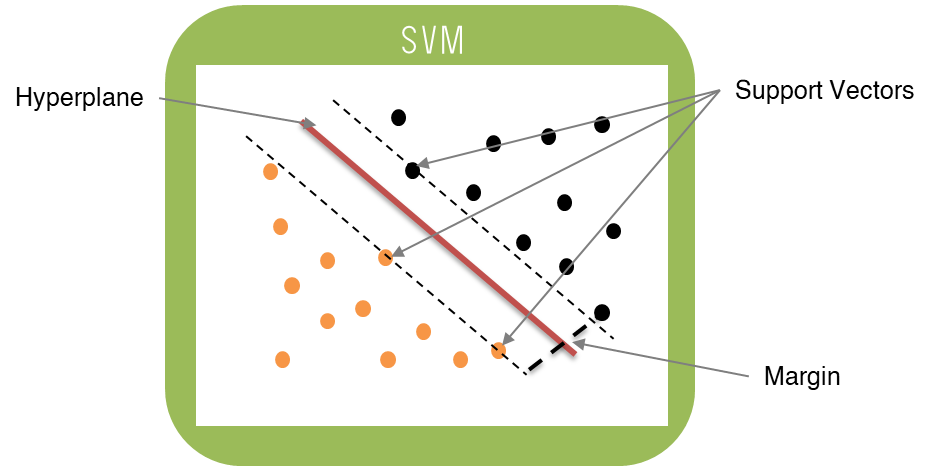
\includegraphics[width=0.6\linewidth]{./figures/SVM.png}}
\caption{Example of a linear boundary estimated by SVM for a two class problem.}
\label{SVMEx}
\end{figure}

In the learning phase, the basis of SVM is the perceptron. This time, the vector of weights $W$ is estimated ensuring that the margin is maximized between the support vectors of both classes. Support vectors are the data points of both classes which are near the hyperplane. Generally, a parameter $g$ defines the quantities of points that will be taken into account while estimating $W$. The highest is $g$, the less support vectors will be used.
For multiclass problem, the one-versus-the-rest strategy is often used.

The main strength of SVM is what is commonly called the "kernel trick". The idea is to apply a transformation $\phi$ to the dataset in order to work on a space where data are linearly separable. An example of kernel transformation is given by Figure~\ref{KernelEx}.

\begin{figure}[htbp]
\centerline{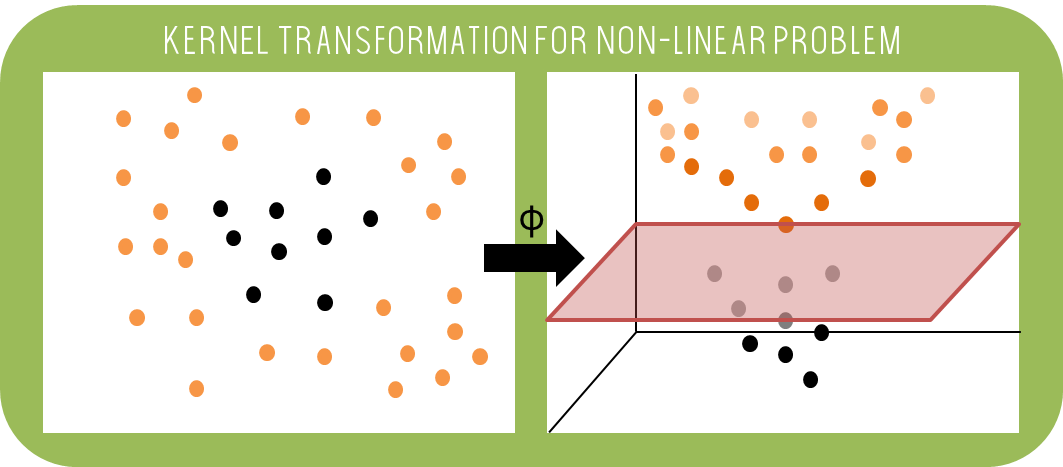
\includegraphics[width=0.75\linewidth]{./figures/KernelTrick.png}}
\caption{Example of kernel transformation $\phi$ and boundary estimation (in red) with SVM.}
\label{KernelEx}
\end{figure}

A wide variety of kernel transformations can be used such as polynomial, radial basis function or sigmoid as well as customized kernels.

Support Vector Machines is a widely used machine learning algorithm. Contrary to RF, it is robust to extreme cases since the hyperplane boundary is computed from support vectors. The main drawback of SVM is that a lot of parameters, depending on the kernel, has to be tuned and finding the best set of parameters can be computationally expensive.

\subsubsection{Multi-Layer Perceptron}

Multi-Layer Perceptron (MLP) is a feedforward artificial neural network. Although a sole perceptron is limited to linear situations, Artificial Neural Networks (ANN) have been constructed in order to solve non-linear problems. There are composed by one input layer, at least one hidden layer and one output layer. Hidden layers and output layers are made up of perceptrons that are all connected from a layer to another. Figure~\ref{MLPEx} depicts an example of MLP with two hidden layers.

\begin{figure}[htbp]
\centerline{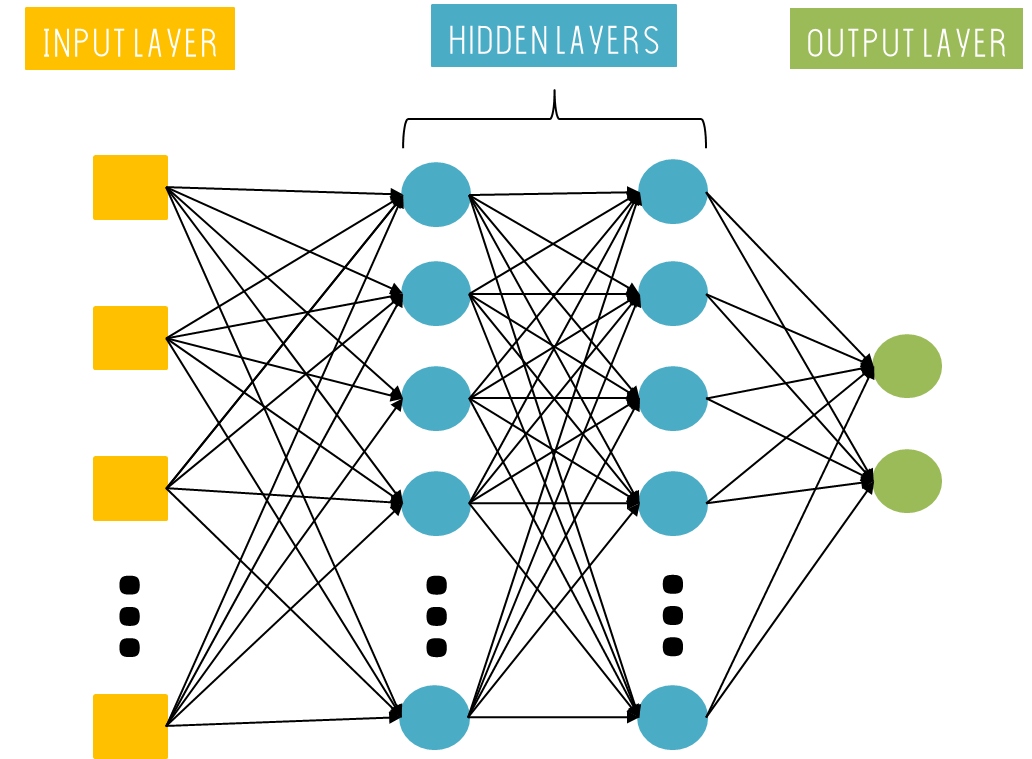
\includegraphics[width=0.75\linewidth]{./figures/MLP.png}}
\caption{Example of multi-layer perceptron with 2 hidden layers and two output classes.}
\label{MLPEx}
\end{figure}

Predictions are made by feeding the feature set of a sample to the network. Then, perceptrons are progressively activated (or not) until reaching an output node which gives the predicted class. Contrary to the linear case, the activation function of each perceptron is non-linear. Among them, we can cite hyperbolic tangent, rectified linear unit function or sigmoid \footnote{Note that in LR, a sigmoid was also used and LR was classified as a linear model. In fact, the output of LR can be written in a linear form whereas, because of the multiple perceptrons, it is not possible to write a linear equation to summarize neural networks outputs. Thus, Neural Networks are classified as non-linear models.}.

For the learning phase, MLP uses a supervised technique called backpropagation. As for the linear case, all samples are passed through the network and weights $W$ are updated according to the output error \cite{parizeau2004perceptron}.
Weights of each perceptron are updated one-by-one, starting from the ones of the output layer.

Neural network is a field in expansion notably because of improvement in computing capacities. Nowadays, neural networks can be composed of a large amount of hidden layers, increasing their depth. This increase of the computing capabilities leads to an evolution of  Neural Networks (e.g., Convolutional Neural Networks, Recurrent Neural Networks) to what is today commonly called deep learning. The main drawback of neural networks is that it involves a lot of parameters to tune (e.g., number of layers, number of perceptrons per layer, connections between layers). In addition, it is also subject to overfit if the training set is too small or not representative of the whole population.
Although today, various complex problems can be solved with deep learning, it is important to remind that it exists alternatives (e.g.,SVM, RF) that are faster, easier to train and can provide better performances regarding the classification objective.

\section{Techniques for performance evaluation}
\label{Evaluation}

As briefly mentioned in Section \ref{Formulation}, evaluation strategies can change regarding the classification objectives, as well as considering the available data. This section firstly focuses on the metrics that are used to evaluate the performances. Secondly, we will go through different techniques used to split an annotated dataset in order to ensure good results for future predictions.

\subsection{Metrics}
\label{metrics}

Parameters and hyper-parameters of machine learning algorithms are tuned by maximizing the performances metrics. Additionally, performance metrics are mandatory to compare the results of different classifiers. In practice, most of performance metrics are based on the confusion matrix, reporting the number of good classifications and misclassifications by comparing the predicted with actual labels. A confusion matrix for a two class problem is reported in Figure~\ref{MC}. It is composed of four numbers:
\begin{itemize}
\item True Positive $TP$: number of samples correctly classified as yes;
\item True Negative $TN$: number of samples correctly classified as no;
\item False Positive $FP$: number of samples classified as 'yes' instead of no;
\item False Negative $FN$: number samples classified as 'no' instead of yes.
\end{itemize}

\begin{figure}[htbp]
\centerline{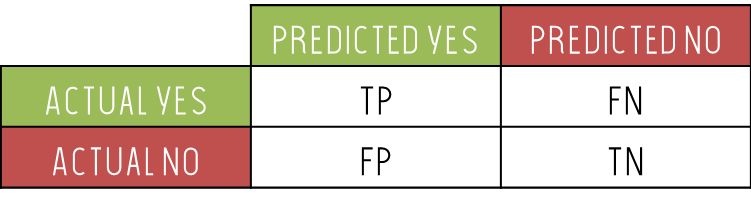
\includegraphics[width=0.5\linewidth]{./figures/ConfusionMatrix.png}}
\caption{Confusion matrix for a two class classification.}
\label{MC}
\end{figure}

From there, the overall classification accuracy $Acc$ measures the total of good classification over the whole data set:
\begin{equation}
Acc = \frac{TP+TN}{TP+FP+TN+FN}
\end{equation}

Measuring the accuracy of a classification is important to give an insight on what the algorithm is capable of. However, it is not always the best way of looking. In fact, for example, in case of imbalanced dataset, a class can take the lead on the accuracy metric and a very high value can be observed even if a less represented class is never detected. Actually, it is often the case in biomedical engineering, notably when working on rare incident diseases. For example, for disease screening, it may be better to hand up with some false positive cases than missing one patient.
Reversely, in some cases, it may be more important to be sure that samples predicted as belonging to a class really belongs to this class.

For these reasons, it exists a bunch of metrics which analyze the performances in different ways. A list of the more common ones is provided hereafter.

Historically, sensitivity and specificity are used to precise classification results:
\begin{itemize}
\item Sensitivity $Se$, which measures the proportion of actual positives that are correctly identified as such:
\begin{equation}
Se = \frac{TP}{FN+TP}
\end{equation}
\item Specificity $Sp$, which measures the proportion of actual negatives that are correctly identified as such:
\begin{equation}
Sp = \frac{TN}{FP+TN}
\end{equation}
\end{itemize}

Recently, with the gain of popularity of machine learning, recall, precision and F-scores are commonly used:

\begin{itemize}
\item Recall $R$, corresponds to $Se$:
\begin{equation}
R = \frac{TP}{FN+TP}
\end{equation}
\item Precision $P$, also known as the Positive Predictive Value (PPV), which measures the fraction of actual positives among the retrieved positive cases:
\begin{equation}
P = \frac{TP}{TP+FP}
\end{equation}
\item F1-score $F_1$ is the harmonic mean of precision and recall and allows a single measure of performance:
\begin{equation}
F_1 = \frac{2 \cdot P \cdot R}{P + R}
\end{equation}
\item $F_\beta$ score, which is the weighted (according to $\beta$) harmonic average of precision and recall:
\begin{equation}
F_{\beta} = \frac{(1+ \beta)^2 \cdot (P \cdot R)}{(\beta^2 + P + R)}
\end{equation}
\end{itemize}

All these metrics are bounded between 0 and 1, where a value of one means a perfect score.
Until there, it may seem that these metrics are only applied on two class problems. However, all these performance measurements can be generalized to multiclass problems, notably by constructing a confusion matrix of one-versus-the-rest for each class.

%\paragraph{Inter-scorer metrics}

%Additionally, two coefficients, historically used to measure inter-scorer reliabity can be computed: the Cohen's Kappa coefficient and the Kendall's tau coefficient.

%The Cohen's Kappa coefficient $\kappa$ that measures a ratio-scaled degree of disagreement between two approaches by taking into account the possibility that it happens by chance \cite{cohen1960coefficient} can be computed. It is defined as follows:
%\begin{equation}
%\kappa = \frac{p_o - p_e}{1-p_e)}
%\end{equation}
%where $p_o$ is the relative observed agreement between predictions and labels, in other words, the accuracy, and $p_e$ is the hypothetical probability of chance agreement, computed as:
%\begin{equation}
%p_e = p_{yes} + p_{no}
%\end{equation}
%with
%\begin{equation}
%p_{yes} = \frac{TP+FN}{TP+FN+TN+FP}
%\end{equation}
%and
%\begin{equation}
%p_{no} = \frac{FP+TN}{TP+FN+TN+FP}
%\end{equation}
%The coefficient $\kappa$ can then be discussed regarding a scale of seven levels, reported in Figure~\ref{Kappa}.
%
%\begin{figure}[htbp]
%\centerline{\includegraphics[width=0.3\linewidth]{./MethodsClassification/figures/Kappa.png}}
%\caption{Scale of Cohen's Kappa coefficient.}
%\label{Kappa}
%\end{figure}
%
%Nevertheless, it may not be enough to understand what kind of errors is made by classifiers. To this end, the Kendall's tau coefficient \cite{kendall1938new} can be calculated. It assesses the rank correlation between two scores and is defined as:
%\begin{equation}
%K_\tau = \frac{(\mbox{number of concordant pairs)} - \mbox{(number of discordant pairs)}}{n(n - 1)/2}
%\end{equation}
%where $n$ is number of evaluated samples.
%
%
%The highest is the Kendall's tau coefficient, the better is the relationship between prediction and labels.

\subsection{Cross-validation}

In order to validate the classifier abilities to make future predictions,
several evaluation strategies can be followed. Cross-validation is the most popular method that helps to ensure the robustness of a classifier  since it allows the detection of underfitting or overfitting \cite{dangeti2017statistics}.
In this section, three popular techniques of cross-validation are presented: Hold-out, K-fold cross-validation and Leave-one-out cross-validation.

\subsubsection{Hold-out}

The hold-out method is the simplest cross-validation technique. Data is divided into two parts: the training set and the testing set, as depicted by Figure~\ref{holdout}.
\begin{figure}[htbp]
\centerline{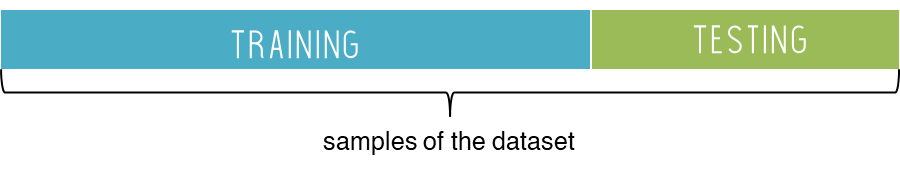
\includegraphics[width=0.8\linewidth]{./figures/holdout.png}}
\caption{Illustration of the hold-out strategy.}
\label{holdout}
\end{figure}
This way, the classifier is trained on the training set and can be evaluated on unseen data of the testing set. Usually, a larger part of the data is used for training. There is two different ways to divide the data: by randomly selecting a number of samples over the whole dataset or by randomly selecting a number of samples of each class, in order to ensure a representation of all classes in the training and in the testing set.
This method is usually applied for small datasets.

\subsubsection{k-fold cross-validation}

One way to improve the hold-out strategy is to perform a $k$-fold cross-validation to tune the parameters and train the model. The idea is to train the model on $k$ different data splits to ensure its robustness.
For each iteration, a training set and a validation set are constructed.
An example of 3-fold cross-validation is provided by Figure~\ref{kfold}.

\begin{figure}[htbp]
\centerline{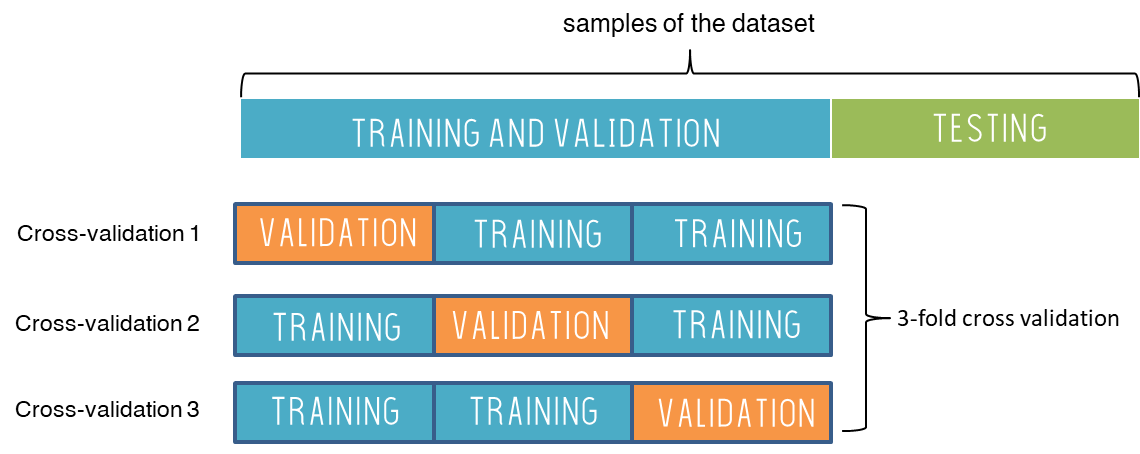
\includegraphics[width=0.8\linewidth]{./figures/kfold.png}}
\caption{Illustration of the 3-fold cross-validation strategy.}
\label{kfold}
\end{figure}

For better control on the classifier performances, it is also recommended to work with an additional set, that wasn't seen during the learning phase and the tuning of the parameters. This set is called the testing set. Hence, in Figure~\ref{kfold}, the 3-fold cross-validation step is only performed on a part of the data.

\subsubsection{Leave-one-out cross-validation}

Leave-one-out cross-validation (LOOCV) is the extreme k-fold validation, where $k$ is equal to the number of samples in the training/validation dataset. An example of LOOCV is depicted by Figure~\ref{LOOCV}.

\begin{figure}[htbp]
\centerline{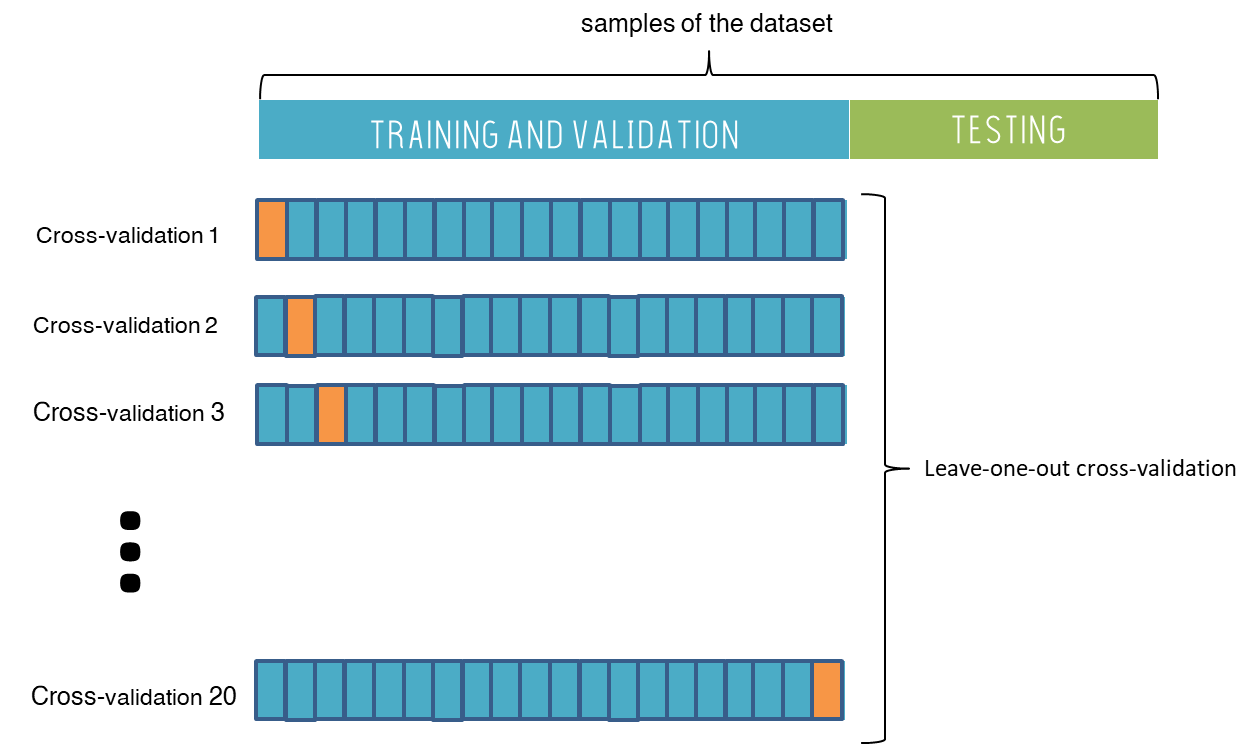
\includegraphics[width=0.8\linewidth]{./figures/loocv.png}}
\caption{Illustration of the leave-one-out cross-validation strategy for a training/validation dataset of 20 samples.}
\label{LOOCV}
\end{figure}

Another way to perform LOOCV exists in biomedical engineering. In fact, to 
evaluate the capacity of classifiers to work with a new patient, a leave-one-patient-out strategy is often performed by working on all patients except one at each time. Performances for each draw indicate the generalization of the model to make future predictions for a new patient.

\section{Conclusion}
Here, key concepts of machine learning for classification were presented. Hence, the process of designing a new classifier was described. It goes from the data collection to the deployment of a new model to make future predictions. We saw that at each step of the design there are some considerations to keep in mind to avoid the construction of non-generalized classifiers. Ensuring the robustness of a model can be done either by carefully selecting or extracting relevant features or by correctly tuning classifier regarding our objective as well as using an accurate evaluation strategy. 

However, the main issue remains the construction of an informative database. In fact, if the dataset is not representative of the reality, all necessary precautions can be taken to avoid underfitting or overfitting, it will be impossible to get to a generalized model.

%In the following chapters, several classification problems are tackled for: automatic detection of sleep stages, segmentation of motion and cry extraction. 
%Each time, the content of this chapter will be recalled to put into perspective our choices.

\addcontentsline{toc}{section}{Bibliography}
\bibliographystyle{acm}
\bibliography{chapterMethods}
\end{document}